% OneMall Paper Review Summary (LaTeX)
\documentclass{article}
\usepackage[margin=1in]{geometry}
\usepackage{graphicx}
\usepackage[T1]{fontenc}
\begin{document}

\section*{OneMall: One Architecture, More Scenarios --- End-to-End Generative Recommender Family at Kuaishou E-Commerce (2026)}
\textbf{arXiv:2601.21770v2 (cs.IR), 2 Feb 2026.}

\subsection*{Challenges}
\begin{itemize}
  \item \textbf{Unifying multiple e-commerce scenarios in one recommender:} Kuaishou e-commerce spans \emph{product-card}, \emph{short-video}, and \emph{live-streaming} item distributions, with different intent signals and item semantics; the paper targets a single end-to-end generative family across them.
  \item \textbf{Tokenizer requirements are unusually strict:} the ``semantic token'' must preserve real-world semantics \emph{and} encode business-specific relations (e.g., product--product co-purchase and short-video--product watching-to-shopping links) across scenarios.
  \item \textbf{Serving-time constraints with long behavioral funnels:} exposure\,$\rightarrow$\,click\,$\rightarrow$\,buy histories are long; naïvely concatenating sequences makes Transformer inference expensive.
  \item \textbf{Bridging retrieval and ranking:} classic cascaded RecSys optimize a retrieval objective and a ranking objective separately; closing that gap requires a stable training pipeline to connect them.
\end{itemize}

\subsection*{Key Initiatives}
\begin{itemize}
  \item \textbf{E-commerce semantic tokenizer (multi-scenario):} learn item representations with an LLM-style multimodal backbone, then quantize to multi-level Semantic IDs (Res-Kmeans + FSQ) with scenario-specific embedding choices.
  \item \textbf{Pure Transformer-based decoder-only architecture:} use Query-Former compression for long user/item feature sequences, cross-attention for multi-behavior fusion, and Sparse MoE to scale total parameters while limiting activated parameters.
  \item \textbf{Retrieval--ranking connection via post-training RL:} use an online ranking model as a reward model and apply preference-optimization style RL (e.g., DPO/GRPO-family) on top of next-token (next-SID) training.
  \item \textbf{Industrial deployment at scale:} the system is reported as deployed and ``serving over 400 million daily active users'' and delivering GMV lifts in multiple surfaces.
\end{itemize}

\subsection*{Methodology}
\begin{itemize}
  \item \textbf{Semantic compression backbone (multimodal embedding):} the tokenizer first fine-tunes an LLM-style multimodal model using Item2Item alignment signals:
    \begin{itemize}
      \item \emph{Inputs:} product main image (224$\times$224) + title; short-video samples 6 frames (224$\times$224) + title/OCR/ASR.
      \item \emph{Backbone choices (as described):} Swin-Transformer as vision encoder and Qwen2.5-1.5B as the text encoder; the last hidden state of a special token \texttt{<EMB>} is used as the final item representation.
      \item \emph{Objective:} InfoNCE-style in-batch contrastive learning on mined positive pairs (product--product, short-video--product).
    \end{itemize}

  \item \textbf{Semantic ID generation (quantization):} convert continuous embeddings to discrete Semantic IDs via a multi-stage pipeline (Figure~\ref{fig:tokenizer}).
    \begin{itemize}
      \item \emph{Res-Kmeans residual quantization:} apply residual K-means codebooks for the first quantization layers.
      \item \emph{FSQ last layer:} a 16-bit quantizer (4096 codes) on the residual is used to reduce code collisions and improve code distribution regularity.
      \item \emph{Scenario-specific embedding candidates:} product-card uses the product embedding; short-video concatenates product + short-video embeddings; live-streaming uses an item-tower embedding plus real-time selling product Semantic IDs as additional features.
    \end{itemize}

  \item \textbf{Decoder-only generative recommender:} the model autoregressively predicts multi-level Semantic IDs, while reducing sequence costs with Query-Former compression and fusing multiple behaviors with cross-attention (Figure~\ref{fig:backbone}). Sparse MoE is used to scale parameters (the paper reports scaling up to 1.3B total parameters with 0.1B activated).

  \item \textbf{RL post-training for retrieval--ranking connection:} the paper treats the online ranking model as a reward model, and optimizes the generator with preference-based RL variants; in their RL setting they mention candidate generation with beam size 768 and balancing NTP and RL losses.
\end{itemize}

\begin{figure}[h]
  \centering
  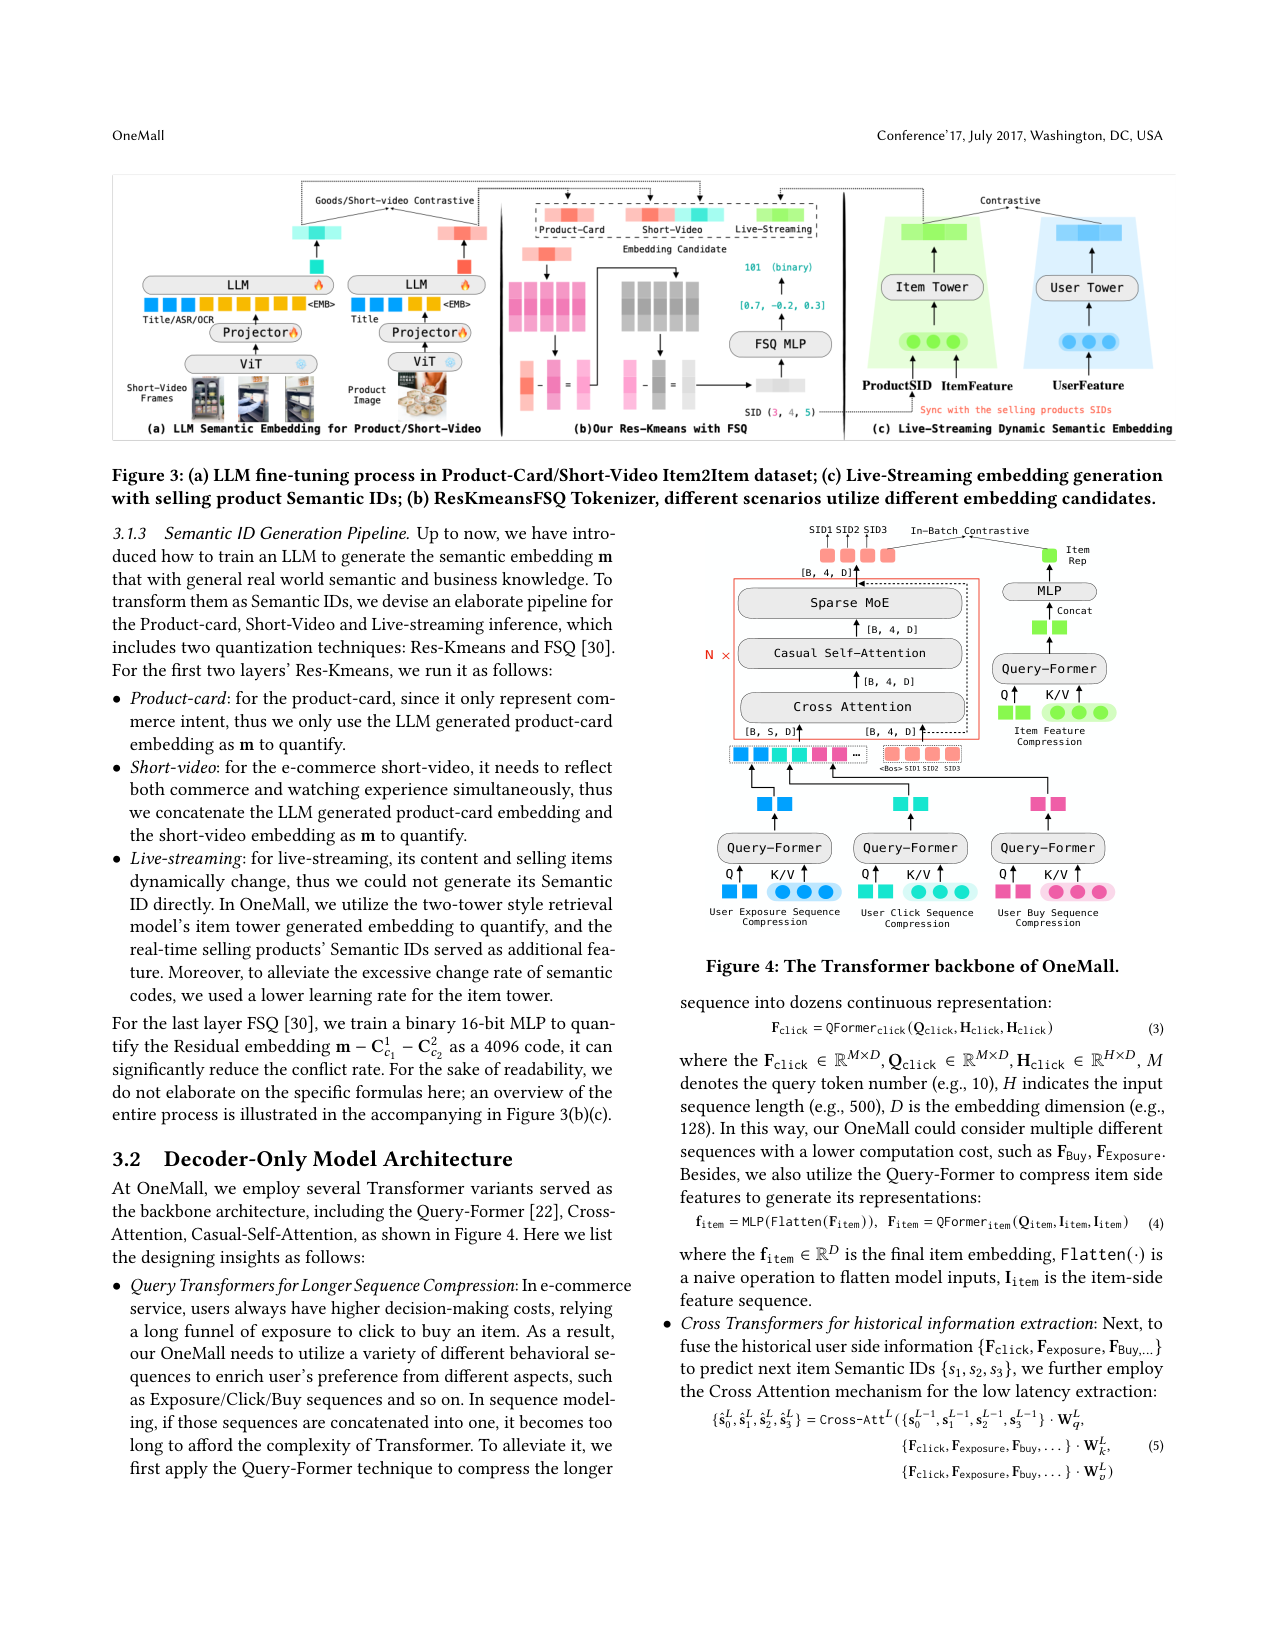
\includegraphics[width=\linewidth]{fig3_tokenizer.png}
  \caption{Tokenizer overview from the paper (Figure 3): LLM-based semantic embedding + ResKmeansFSQ semantic IDs across scenarios.}
  \label{fig:tokenizer}
\end{figure}

\begin{figure}[h]
  \centering
  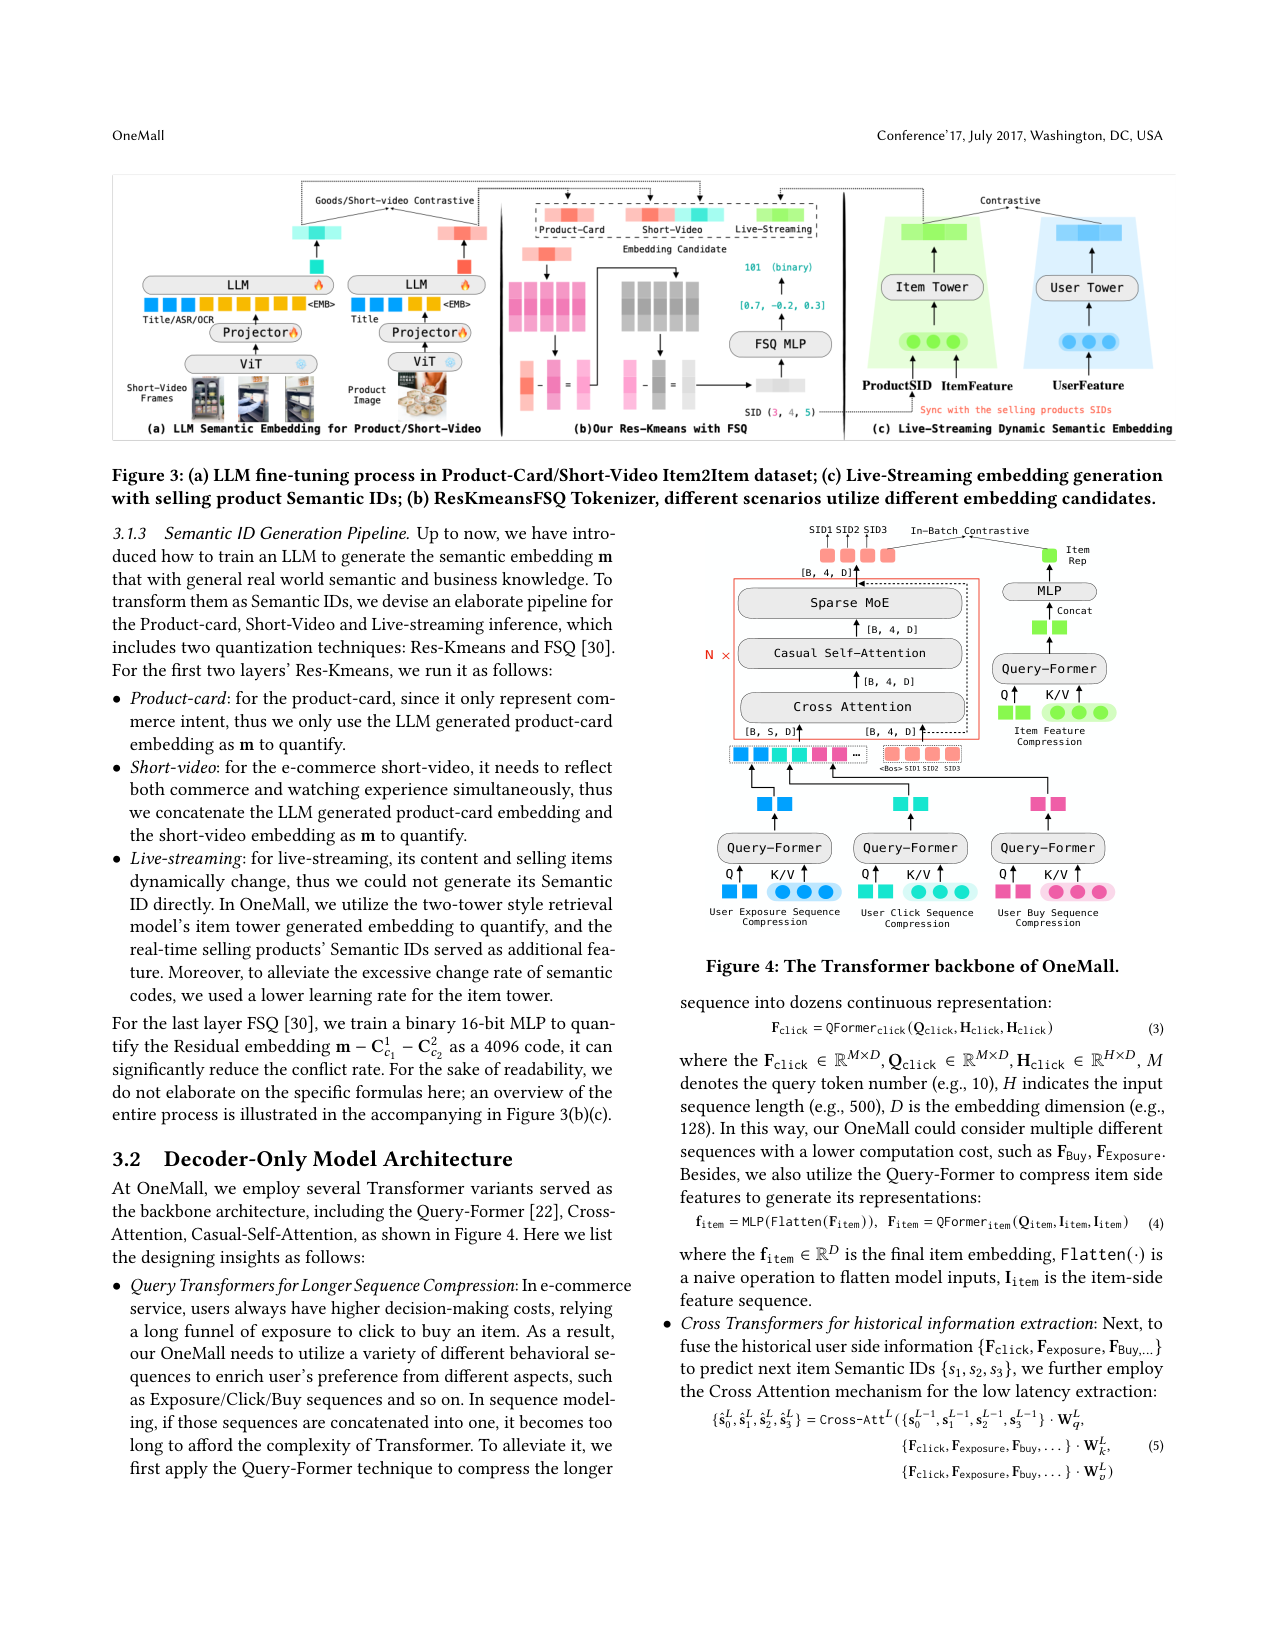
\includegraphics[width=\linewidth]{fig4_transformer_backbone.png}
  \caption{Transformer backbone from the paper (Figure 4): Query-Former compression + cross-attention fusion + decoder-only SID generation.}
  \label{fig:backbone}
\end{figure}

\subsection*{Experiments}
\begin{itemize}
  \item \textbf{Offline scaling (short-video scenario):} as total parameters scale from 0.05B to 1.3B-A0.1B, the paper reports Acc-SID1/2/3 improving from 14.5\%/43.9\%/61.0\% to 16.2\%/51.7\%/71.7\%, and simulation HR@50/100/500 improving from 32.9\%/41.3\%/60.5\% to 45.6\%/57.3\%/76.0\% (Table 1).
  \item \textbf{Simulation replay vs baselines:} OneMall (0.5B-A0.1B) outperforms SASRec and TIGER across product-card / short-video / live-streaming scenarios; e.g., Product-card HR@50 improves to 34.3\% vs 23.2\% (SASRec) and 29.5\% (TIGER), and Live-streaming HR@500 improves to 80.5\% vs 68.4\% (SASRec) and 73.7\% (TIGER) (Table 2).
  \item \textbf{Online A/B impact (business metrics):} the abstract highlights ``+14.7\% GMV in Product-Card, +10.3\% GMV in Short-Video, and +4.9\% GMV in Live-Streaming''; later, Table 3 reports detailed lifts (e.g., Product-Card +14.71\% GMV; Short-Video +10.33\% GMV; Live-Streaming +4.90\% GMV).
  \item \textbf{RL effectiveness:} DPO/GRPO improve CTR/CTCVR/GPM over the base model across multiple candidate segments, and GRPO is reported stronger than DPO in their setting (Table 4).
  \item \textbf{Component analyses:} adding FSQ reduces tokenizer conflict (Table 5); Query-Former drastically reduces sequence length and GFLOPs with minor hit-rate changes (Table 6); an auxiliary contrastive objective improves HR metrics by about +1.5\%/+1.7\%/+1.7\% on HR@50/100/500 (Section 4.5).
\end{itemize}

\subsection*{References (selected; cited/used by the paper)}
\begin{itemize}
  \item Scaling laws / LLM training: OpenAI (GPT-4 technical report), Achiam et al., 2023.
  \item Generative retrieval in RecSys: TIGER, Rajput et al., 2023.
  \item Sequential recommendation baseline: SASRec, Kang and McAuley, 2018.
  \item Vision--language pretraining components: BLIP-2 / Query-Former, Li et al., 2023.
  \item Contrastive learning objective: InfoNCE / CPC, van den Oord et al., 2018 (as referenced by the paper).
  \item Finite Scalar Quantization (FSQ): Mentzer et al., 2023.
  \item Preference optimization / RL: DPO (Rafailov et al., 2023), PPO (Schulman et al., 2017).
  \item Distributed training techniques: ZeRO (Rajbhandari et al., 2020), Tensor parallelism (Shoeybi et al., 2019).
\end{itemize}

\end{document}
